\chapter{Teoretične osnove}

Parametre za iskano hidroelektrarno lahko izračunamo po naslednjem algoritmu:
\begin{enumerate}[noitemsep, topsep=0pt]
	\item Pridobitev podatkov
	\item Analiza hidrološkega niza podatkov za iskano obdobje
	\item Izračun konsumpcijske krivulje
	\item Izračun proizvodnje električne energije
\end{enumerate}


%-------------------------------------
\section{Pridobitev podatkov}
Za nadaljnje izračune potrebujemo podatke o:
\begin{itemize}[noitemsep, topsep=0pt]
	\item Dimenzijah in naklonu rečne struge
	\item Manningovem koeficientu hrapavosti rečnega korita
	\item Povprečnih dnevnih pretokih vodotoka za izbrano obdobje
\end{itemize}

Podatke o dimenzijah rečnega korita lahko pridobimo z meritvami na terenu ali pa dimenzije ocenimo na podlagi ortofoto posnetkov. Naklon rečne struge vodotoka se lahko oceni s pomočjo spletne aplikacije Geopedija. Izberemo odsek vodotoka, ki ga definirata dve točki. S pomočjo Geopedije odčitamo podatke o višinski razliki $\Delta h$ in razdalji $\Delta L$ med točkama. S pomočjo spodnje enačbe določimo naklon izbranega odseka vodotoka:

\begin{ceqn}
\begin{align}
 I = \dfrac{100\Delta h}{\Delta L} [\%]
\end{align}
\end{ceqn}


  Manningov koeficient hrapavosti rečnega korita $ng$ se lahko oceni izkustveno na terenu s pomočjo priročnikov ali pa z umerjanjem na podlagi podatkov o nivojih vode in pretokih. Manningov koeficient hrapavosti je odvisen od naslednjih 7 faktorjev \cite{VenTeChow}:
 \begin{enumerate}[noitemsep, topsep=0pt]
 	\item Hrapavosti površine ostenja
 	\item Zaraščenosti rečnega korita
 	\item Neregularnosti oblike rečnega korita
 	\item Meandriranja rečne struge
 	\item Zamašitve struge s plavinami 
 	\item Oblike in velikosti rečnega korita
 	\item Polnosti korita z vodo
 \end{enumerate}
 

 
 
  Podatke o pretokih slovenskih vodotokov lahko pridobimo iz arhiva, ki se nahaja na spletni strani agencije Republike Slovenije za okolje (v nadaljevanju ARSO). V primeru da iščemo pretok za manjši vodotok, je zelo verjetno da podatki o pretokih vodotoka ne obstajajo. V tem primeru lahko pretok vodotoka ocenimo s pomočjo meritev višine gladine vode in dimenzij struge, ocene Manningovega koeficienta hrapavosti in naklona struge. S pomočjo Manningove enačbe opisane kasneje v poglavju~\ref{sec:teorija_trapeznaMetoda} in prej omenjenih členov Manningove enačbe dobimo končno ocenjeno vrednost pretoka vodotoka za posamezno obdobje meritev.




%------------------------------------------------
\section{Analiza hidrološkega niza podatkov}
%TODO: FIXME -> izboljšaj
Iz ARSO-vega arhiva lahko izvozimo podatke o povprečnih dnevnih pretokih iskanega vodotoka v csv obliki (comma separated values). Iz izvoženih podatkov lahko za vsak mesec obdobja izračunamo povprečni mesečni pretok. Če mesečne pretoke povprečimo za vsa leta izbranega obdobja lahko navedene povprečne mesečne pretoke obdobja prikažemo na hidrogramu obdobja. Hidrogram je graf, ki prikazuje povprečne mesečne pretoke vodotoka za izbrano obdobje analize.  %Prav tako se lahko določi mokro in suho leto obdobja, ki ju primerjamo s povprečnimi mesečnimi pretoki.

%TODO: krivulja trajanja



%------------------------------------------------
\section{Izračun konsumpcijske krivulje}
Konsumpcijska krivulja je graf funkcije, ki predstavlja višino gladine vode v odvisnosti od pretoka vode v rečni strugi. Graf konsumpcijske krivulje potrebujemo za določitev višinske razlike $dh$ med spodnjo in zgornjo vodo hidroelektrarne v odvisnosti od pretoka vode skozi turbine hidroelektrarne. Višinsko razliko $dh$ potrebujemo za določitev moči hidroelektrarne v zadnjem koraku algoritma opisanega v tem poglavju.



%-------------------------------------------------
\subsection{Izračun konsumpcijske krivulje za pravokotne in trapezne struge} \label{sec:teorija_trapeznaMetoda}
Za izračun konsumpcijske krivulje potrebujemo pretok vodotoka $Q$ v odvisnosti od višine gladine vode $h$ v strugi. Gladina vode $h$ poteka od dna struge do maksimalne višine struge vodotoka $H$. Pretok vode v strugi $Q$ se za vsak cm višine $h$ izračuna po Manningovi enačbi:

\begin{ceqn}
\begin{align}
Q(h) = \dfrac{1}{ng} \sqrt{I}\dfrac{S(h)^{5/3}}{P(h)^{2/3}} \label{eq:ManningovaEnacba}
\end{align}
\end{ceqn}

Kjer je:

\begin{table}[htb!]
	\begin{tabular}{r|p{10cm}}
		Q & pretok \\
		ng & Manningov koeficient hrapavosti dna struge\\
		I & naklon struge \\
		S & ploščina omočenega dela prečnega profila \\
		P & dolžina omočenega oboda struge
	\end{tabular}
\end{table}


\newpage
% pravokotna struga
\begin{enumerate}
	\item Pravokotno oblikovana struga vodotoka:
	
	\begin{figure}[H]
		\begin{centering}
			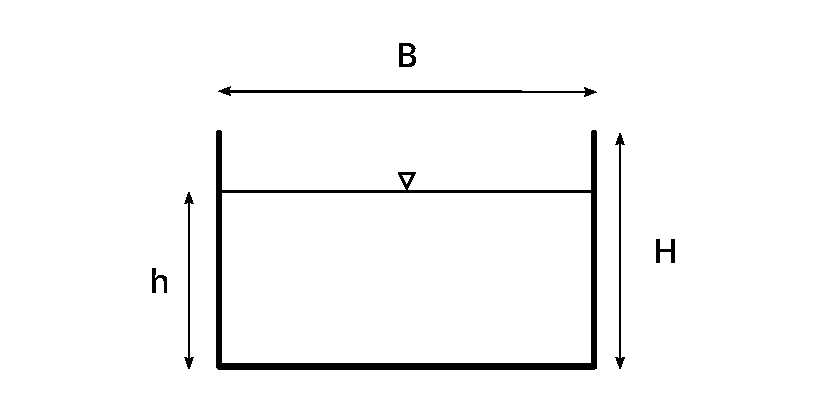
\includegraphics{slike/konsumpcijska_krivulja/rectangularChannel.pdf}		
			\caption{Prečni prerez pravokotne struge}\label{fig:pravokotna struga}
		\end{centering}
	\end{figure}
	

	Omočeni obod pravokotne struge izračunamo kot seštevek širine dna struge in dvakratne višine gladine vode v strugi vodotoka $h$.
	
	\begin{ceqn}
	\begin{equation}
	P_{p}(h) = B + 2h
	\end{equation}
	\end{ceqn}
	
	Ploščino omočenega dela, ki ga omejujejo rečno korito in gladina vode za pravokotno oblikovano rečno strugo dobimo po enačbi:
	
	\begin{ceqn}
	\begin{align}
	S_{p}(h) = B \cdot h
	\end{align}
	\end{ceqn}
	
	\item Trapezno oblikovana struga vodotoka:
	
		\begin{figure}[ht!]
			\begin{centering}
				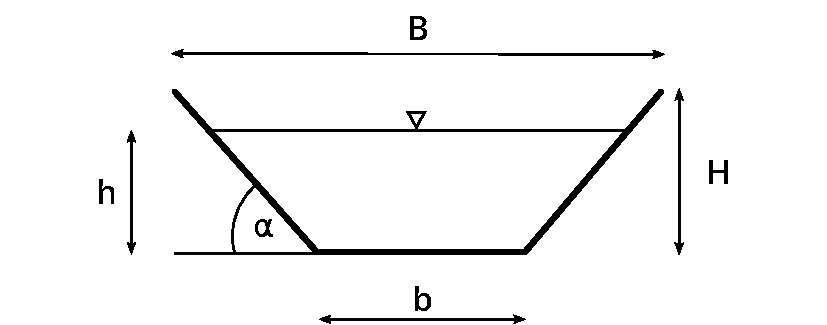
\includegraphics{slike/konsumpcijska_krivulja/trapezoidChannel.pdf}		
				\caption{Prečni prerez trapezne struge}\label{fig:trapezna struga}
			\end{centering}
		\end{figure}
	
	Omočeni obod trapezno oblikovane rečne struge izračunamo kot seštevek širine dna struge in dvakratne razdalje od roba dna do točke presečišča rečnega korita z gladino vode:
	
	\begin{ceqn}
	\begin{align}
	P_{t}(h) = b + 2 \cdot \sqrt{h^2 + \left(\dfrac{h} {\tan\alpha} \right)^{2}}
	\end{align}
	\end{ceqn}
	
	Ploščino omočenega dela v trapezno oblikovani rečni strugi izračunamo po enačbi:
	\begin{ceqn}
	\begin{align}
	S_{t}(h) = b \cdot h + \dfrac{h^2}{ 2\tan\alpha}
	\end{align}
	\end{ceqn}
	
\end{enumerate}



Ko poznamo vse parametre Manningove enačbe \ref{eq:ManningovaEnacba}, izračunamo pretoke vodotoka za vsak cm višine rečne struge, ki poteka od višine 0 do $H$ in narišemo graf konsumpcijske krivulje $h(Q)$.


\newpage
%------------------------------------------------
\subsection{Izračun konsumpcijske krivulje za struge poljubne oblike}\label{sec:pretokNumericnaMetoda}


V primeru da iščemo konsumpcijsko krivuljo za vodotok poljubne oblike, si za izračun le te ne moremo pomagati s znanimi formulami preprostih geometrijskih likov. Poljubno oblikovano strugo lahko popišemo s serijo točk, ki jih dodajamo v kartezijski koordinatni sistem. Za vsako točko ki definira poljubno rečno korito podamo x in y koordinato, za točke pa predpostavimo da so med seboj povezane z enačbo linearne funkcije. Na sliki~\ref{fig:poljubnaStruga} je predstavljen prečni prerez poljubno oblikovane struge vodotoka.

\begin{figure}[ht!]
	\begin{centering}
		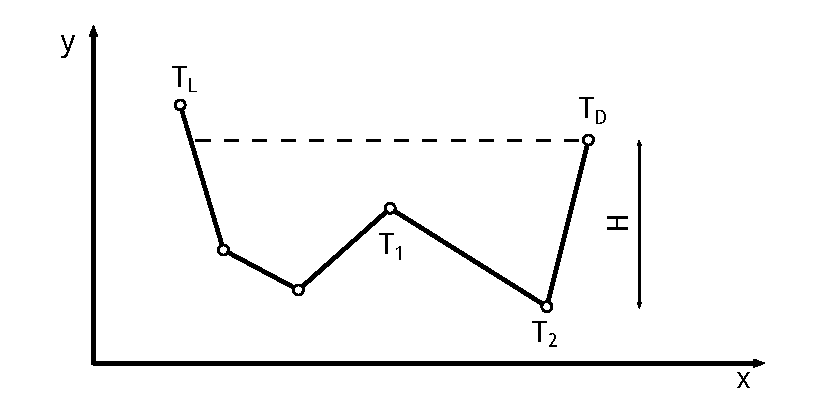
\includegraphics{slike/customChannel/customStruga.pdf}		
		\caption{Prečni prerez poljubno oblikovane struge vodotoka}\label{fig:poljubnaStruga}
	\end{centering}
\end{figure}



%------------------------------------------
%\subsection{Izračun višine rečnega korita}
Skrajni točki na robu struge sta točki $T_L$ in $T_D$ na sliki \ref{fig:poljubnaStruga}. Točko na robu struge z nižjo y koordinato označimo s $T_{Rmin}$ (na sliki \ref{fig:poljubnaStruga} označena kot točka $T_D$). Najnižjo točko struge vodotoka označimo s $T_{min}$. Maksimalna gladina vode v rečnem koritu $H$ je definirana kot razdalja med točkama $T_{Rmin}$ in $T_{min}$. V primeru da je višina gladine vode večja od višine rečnega korita $H$ pride do preliva vode čez robove rečnega korita.



%\subsection{Določitev parametrov odseka}
Za določitev parametrov odseka, ki jih potrebujemo za izračun konsumpcijske krivulje, s točkami definirano poljubno strugo vodotoka najprej razdelimo na odseke po dve točki $O_1$ ($x_1$, $y_1$) in $O_2$ ($x_2$, $y_2$). Za vsak izbran odsek rečne struge, se najprej določi enačba linearne funkcije, ki povezuje točki $O_1$ in $O_2$.

Enačba linearne funkcije se definira kot:
\begin{ceqn}
\begin{align}
f(x) = kx + n \label{eq:enacba_linearnafunkcija}
\end{align}
\end{ceqn}

Naklon funkcije k se izračuna po spodnji enačbi:

\begin{ceqn}
\begin{align}
k = \dfrac{y_2 - y_1}{x_2 - x_1}
\end{align}
\end{ceqn}



Če v enačbo linearne funkcije \ref{eq:enacba_linearnafunkcija} vstavimo izračunan naklon $k$ in koordinate točke $O_1$, lahko izračunamo iskani $n$. S tem je določena enačba linearne funkcije $f(x)$ ki povezuje točki $O_1$ in $O_2$.

\begin{figure}[H]
	\begin{centering}
		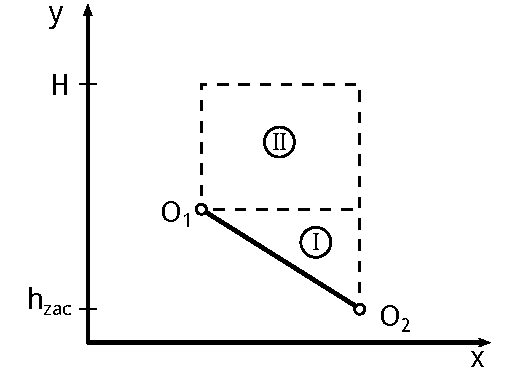
\includegraphics{slike/customChannel/odsek.pdf}
		\caption{Izbrani odsek struge} \label{fig:odsekStruge}
	\end{centering}
\end{figure}








% določitev ploščine posameznega kosa
Za vsak odsek dveh točk se določi najnižja točka odseka $T_{zac}$, na sliki \ref{fig:odsekStruge} označena kot točka $O_2$. Y koordinata točke $T_{zac}$ nam predstavlja začetno višino odseka $h_{zac}$. Od $h_{zac}$ do končne višine rečnega korita H za vsak cm po višini določimo presečišče $P_1$ prej izračunane funkcije $f(x)$ s horizontalno ravnino $g$, ki predstavlja gladino vode pri trenutni višini $h$. Opisani postopek je prikazan na sliki \ref{fig:custom_odsekDetajl}.


\begin{figure}[ht!]
	\begin{centering}
		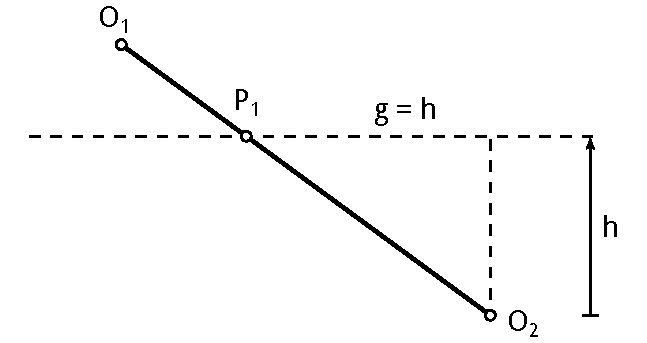
\includegraphics{slike/customChannel/odsek_detajl.pdf}
		\caption{Detajl odseka struge}\label{fig:custom_odsekDetajl}
	\end{centering}
\end{figure}



Ko imamo določeno presečišče $P_1$ gladine vode s funkcijo $f(x)$ med točkama odseka, lahko izračunamo dolžino omočenega oboda struge odseka in ploščino lika ki ga oklepajo funkcija odseka $f(x)$, navidezna gladina vode $g$ in najnižja točka odseka $T_{zac}$ na sliki \ref{fig:odsekStruge} označena z $O_2$.


Način izračuna omočenega oboda struge vodotoka $P(h)$ in ploščine prečnega prereza $S(h)$ je odvisen od pozicije presečišča $P_1$:


\begin{enumerate}
	\item V primeru da se presečišče $P_1$ odseka nahaja v območju med točkama $O_1$ in $O_2$, dolžino omočenega oboda določimo po Pitagorovem izreku kot:
		
	%FIXME: decide on index P_1_x or P_1x
	\begin{ceqn}
		\begin{align}
		P(h) = \sqrt{(T_{zac\_x} - P_{1\_x}(h))^{2} + (T_{zac\_y} - P_{1\_y}(h))^{2}}
		\end{align}
	\end{ceqn}
	
	
	Ploščino območja ki ga oklepajo horizontalna ravnina s presečiščem $P_1$ in najnižjo točko odseka $T_{zac}$ pa določimo kot ploščino trikotnika (območje I na sliki~\ref{fig:odsekStruge}) po formuli:
	
	\begin{ceqn}
	\begin{align}
	S(h) = \dfrac{|T_{zac\_x} - P_{1x}(h)| \cdot |T_{zac\_y} - P_{1y}(h)|}{2}
	\end{align}
	\end{ceqn}
	
	
	\item V primeru, da se presečišče $P1$ nahaja izven območja točk $O_1$ in $O_2$ se dolžina omočenega oboda odseka izračuna kot razdalja med točkama $O_1$ in $O_2$ po Pitagorovem izreku:
	
	\begin{ceqn}
	\begin{align}
	P = \sqrt{ (O_1x - O_2x)^{2} + (O_1y - O_2y)^{2}}
	\end{align}
	\end{ceqn}
	
	Ploščina $S$ odseka pa se določi kot seštevek ploščin območij I in II na sliki \ref{fig:odsekStruge}.
	
	\begin{ceqn}
	\begin{align}
	S(h) = S_I + S_{II}(h)
	\end{align}
	\end{ceqn}
	
	Pri čemer sta $S_I$ in $S_{II}$ enaka:
	
	\begin{ceqn}
	\begin{align}
	S_I&= \bigg|\dfrac{ (O_2y - O_1y) \cdot  (O_2x - O_1x)}{2}\bigg|\\
	S_{II}(h)&= \bigg|(O_{2x} - O_{1x}) \cdot (h - O_{1y})\bigg|
	\end{align}
	\end{ceqn}

	
\end{enumerate}


Ko imamo za vsak cm višine gladine vode izračunan omočeni obod $P_n(h)$ odseka $n$ in ploščino prečnega prereza pod gladino vode $S_n(h)$ lahko določimo pretok vode skozi odsek $Q_n(h)$. Pretok vode skozi odsek izračunamo po Manningovi enačbi \ref{eq:ManningovaEnacba}. Za vsak računani odsek moramo poznati tudi naklon struge vodotoka $I_n$ in  Manningov koeficient hrapavosti površine $ng_n$.


\begin{ceqn}
	\begin{align}
	Q_n(h) = \dfrac{1}{ng_n} \sqrt{I_n}\dfrac{S_n(h)^{5/3}}{P_n(h)^{2/3}}
	\end{align}
\end{ceqn}


Ko imamo posamezne pretoke po višinah za vse odseke izračunane, jih medsebojno seštejemo in dobimo končne vrednosti pretokov $Q(h)$:

\begin{ceqn}
\begin{align}
Q(h) = Q_1(h) + Q_2(h) + Q_3(h) + ... + Q_{n-1}(h) + Q_n(h)
\end{align}
\end{ceqn}


S imamo točke za izris konsumpcijske krivulje določene in funkcijo konsumpcijske narišemo na graf $h(Q)$.



\newpage

\section{Izračun proizvodnje električne energije}
Za določitev končne proizvodnje električne energije potrebujemo razliko med koto zgornje vode t.j. vode v rezervoarju in koto spodnje vode, ki jo določimo iz grafa konsumpcijske krivulje izračunanega za izbrano strugo.

\begin{figure}[ht!]
	\begin{centering}
		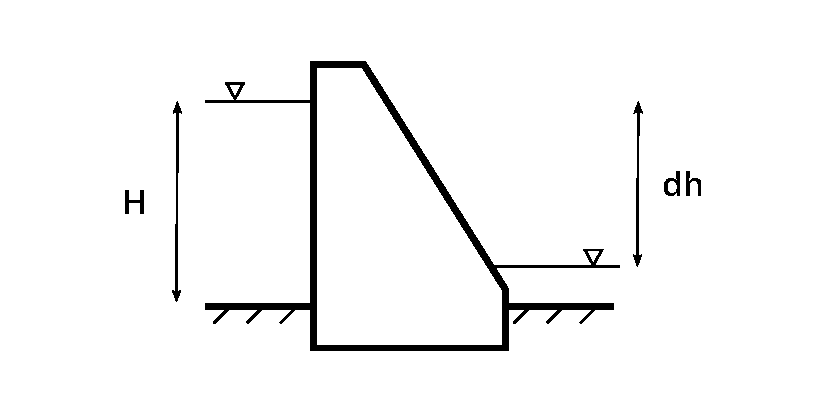
\includegraphics{slike/electricityProduction/powerplant_crossSection.pdf}
		\caption{Shema prečnega prereza hidroelektrarne}
	\end{centering}
\end{figure}

Ker računamo proizvodnjo električne energije za pretočne hidroelektrarne, predpostavimo da je kota zgornje vode konstantna na višini $H$. Koto spodnje vode določimo iz prej izračunane konsumpcijske krivulje iz katere odčitamo višino spodnje vode v strugi za dani povprečni mesečni pretok skozi turbino hidroelektrarne. V primeru da se pretok skozi turbino hidroelektrarne nahaja med dvema točkama pretokov v konsumpcijski krivulji, iskano višino spodnje vode določimo z linearno interpolacijo med znanima točkama na grafu konsumpcijske krivulje.

Višinsko razliko med koto zgornje in spodnje vode določimo po spodnji enačbi:

\begin{ceqn}
\begin{align}
dh = H - H_{spodaj}
\end{align}
\end{ceqn}

Moč hidroelektrarne izračunamo po enačbi:

\begin{ceqn}
\begin{align}
P = \mu \cdot g \cdot Q \cdot dh
\end{align}
\end{ceqn}

Pri čemer so:
\begin{table}[htb!]
	\begin{tabular}{r|p{10cm}}
		P & moč [$kW$]\\
		$\mu$ & izkoristek turbine [\%]\\
		g & gravitacijska konstanta [$9,81\dfrac{m}{s^{2}}$ ] \\
		Q & pretok [$m^{3}/s$]\\
		dh & razlika višin spodnje in zgornje vode [$m$]
	\end{tabular}
\end{table}


Za določitev končne mesečne proizvodnje električne energije, za vsak mesec določimo povprečno moč $\overline{P}$ in uporabimo naslednjo enačbo

\begin{ceqn}
\begin{align}
E = \dfrac{24 \cdot \overline{P} \cdot d}{1000}
\end{align}
\end{ceqn}

Pri čemer so:
\begin{table}[htb!]
\begin{tabular}{r|p{10cm}}
	E & proizvedena električna energija [$MWh$]\\
	$\overline{P}$ & povprečna moč v mesecu [$kW$]\\
	d & število dni v mesecu \\
\end{tabular}
\end{table}

